This section explains the results of the project in \ref{subsec:results} and evaluate on the results in \ref{subsec:evaluation}.

\subsection{Results}
\label{subsec:results}
The Results section contains results for both the preprocessing and the two classification algorithms and their performance.

\subsubsection{Preprocessing}

\begin{figure}
\centering
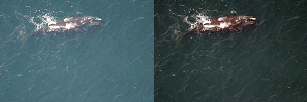
\includegraphics{Images/preprocess1}
\end{figure}






\subsubsection{Random Forest}
The Results for Random Forest is split into two sections. As there has been conducted classification for both data which was just resized and data which has been additionally preprocessed before resizing.

\paragraph{The Resized Data}
\label{par:rf-resized}
shown in Figure \ref{fig:rf-resized}, represent an averaged result of 3 fold cross validation. The Graph is shown with a one-tailed 95\% confident interval with a degree of freedom on 3. The criteria of interest is the potential worst performance of the model. Which is the upper line of the embedded errorbar on the graph at each point. The cutoff line defines the performance at random selection, which is 1 / 447. 

Each validation point for the chart correspond to the number of trees in the forest, plus 1 additional tree. So for validation point ``5'', the model has 6 trees.

The performance of the test set for Figure \ref{fig:rf-resized} do for each validation point have a \emph{significant better performance} than choosing random selection.

The training set does significant better than the test set, but just states that the model is overfitted and should be trained against more observations to introduce more variety.

\begin{figure*}
  \centering
  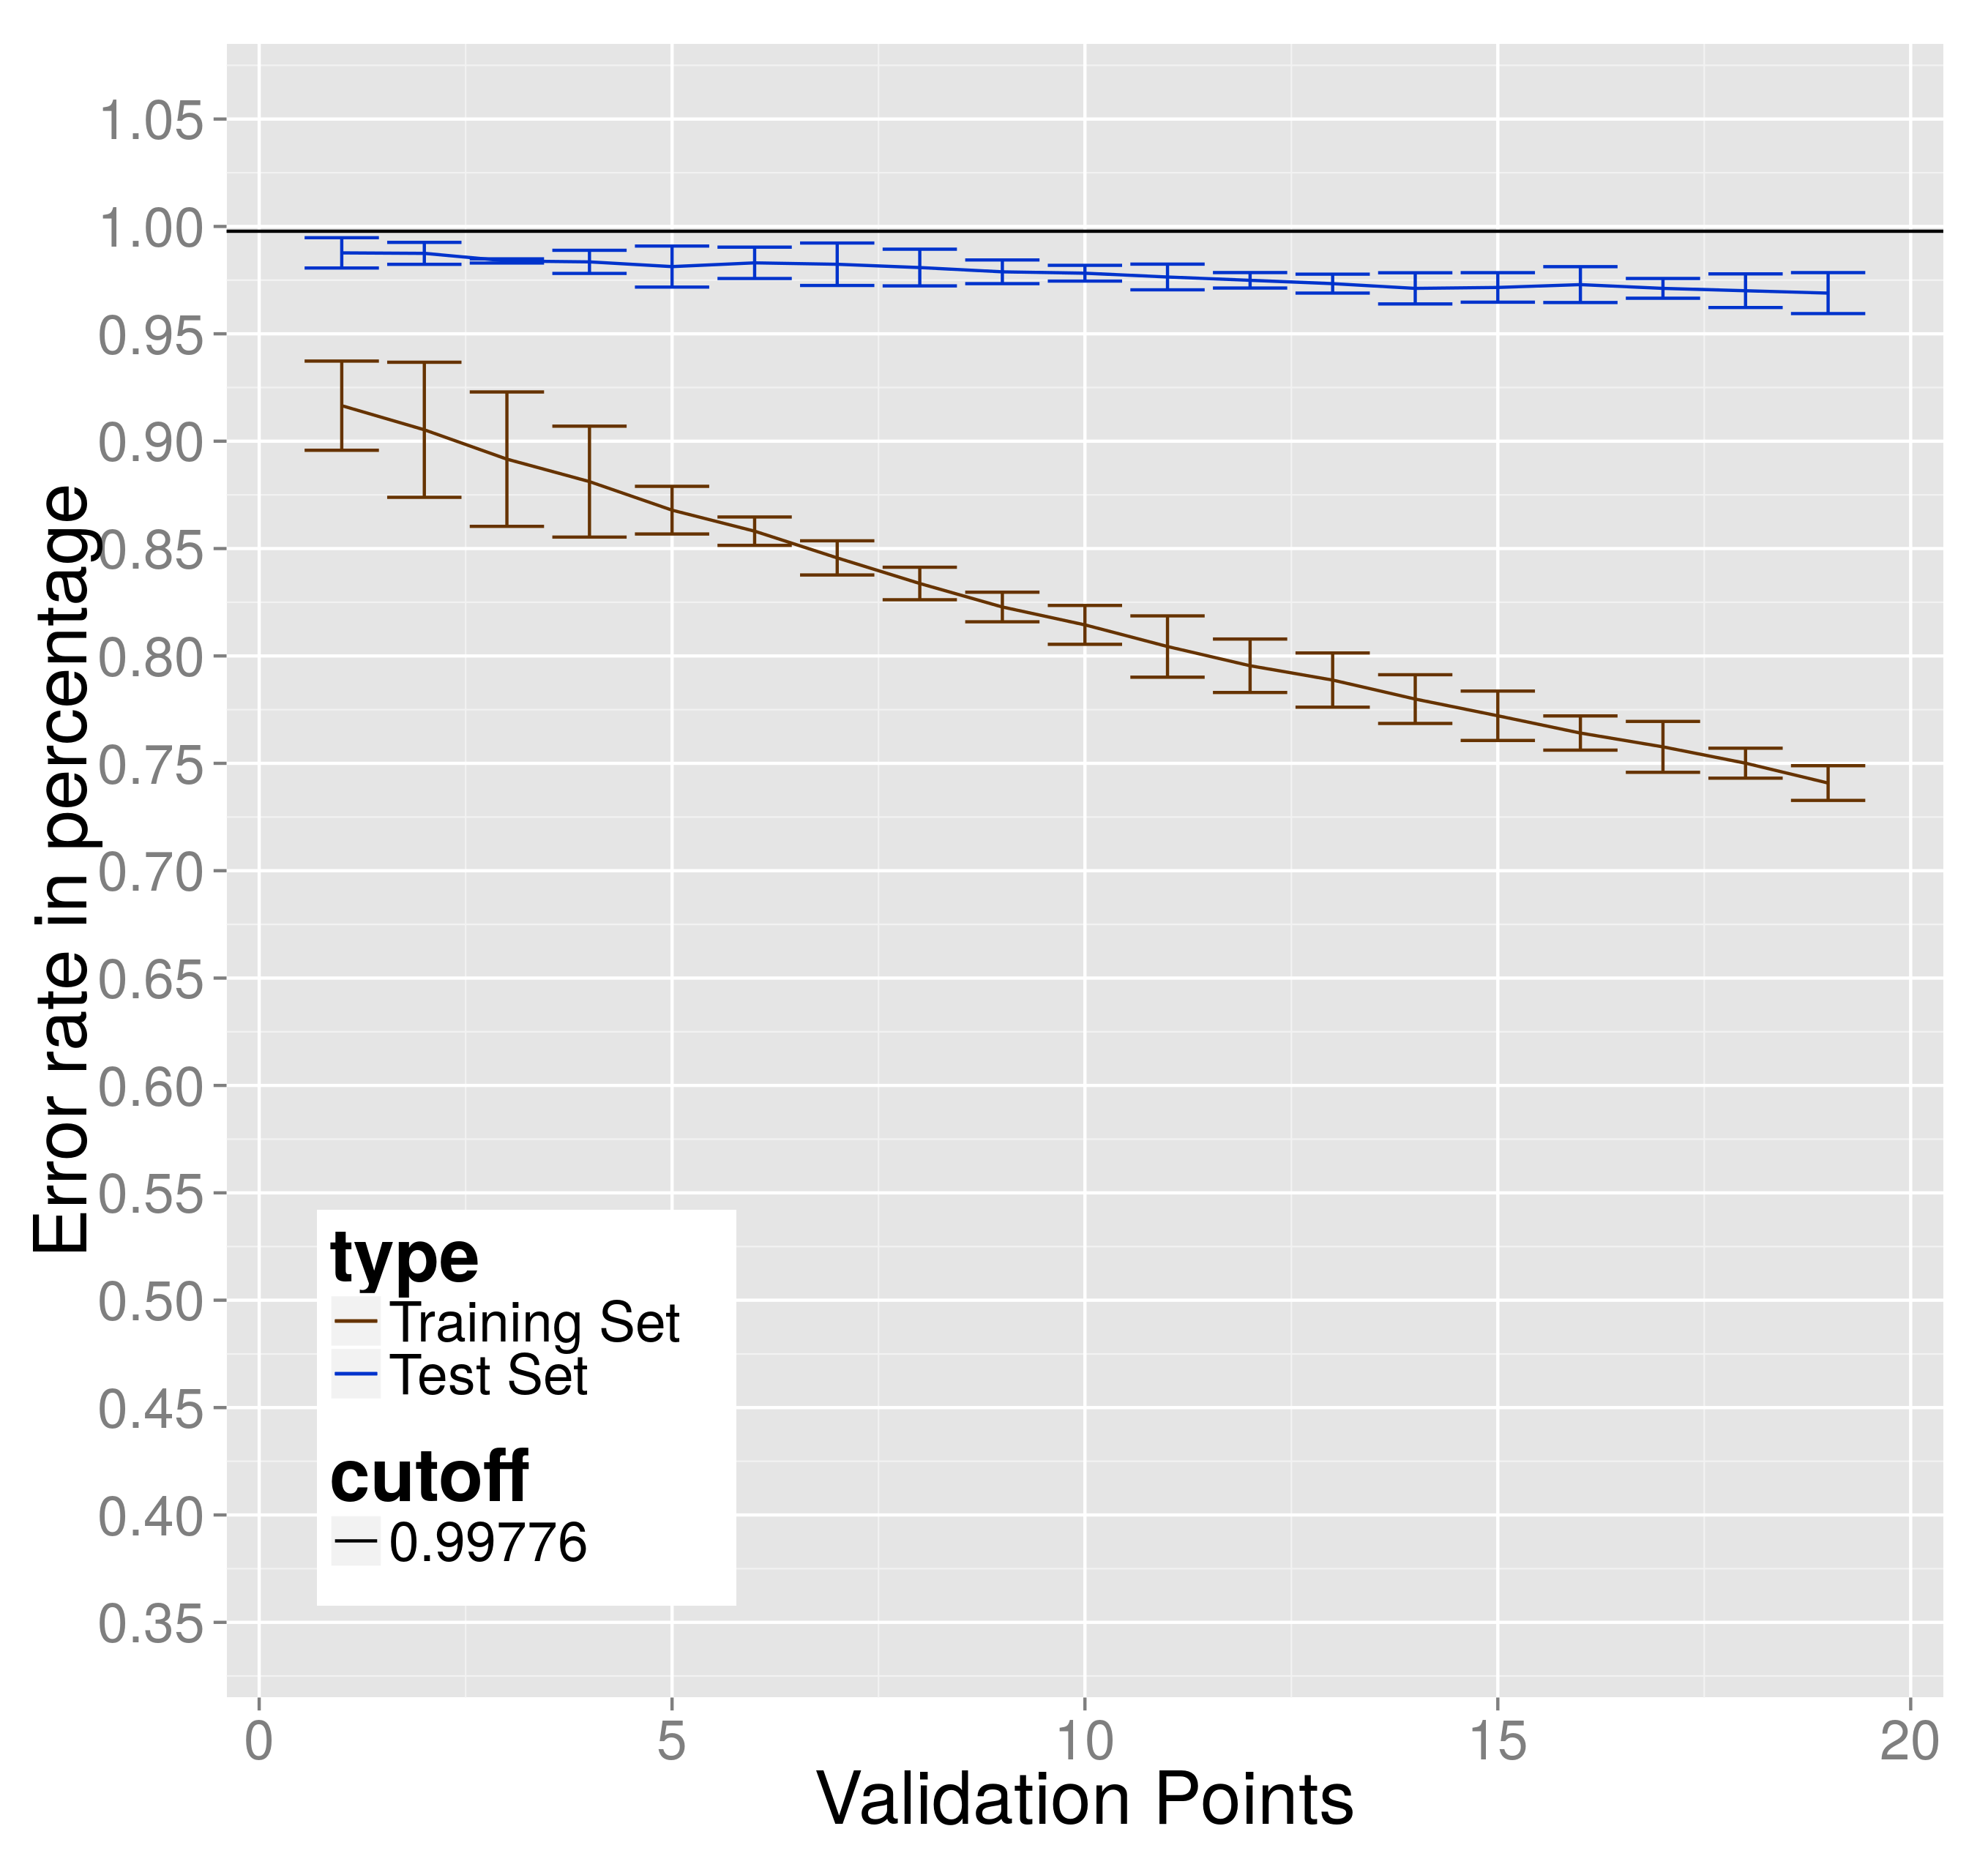
\includegraphics[width=0.9\linewidth]{Images/DRFraw}
  \caption{Random Forest - Resized Images}
  \label{fig:rf-resized}
\end{figure*}

\paragraph{The Preprocessed Data}
shown in Figure \ref{fig:rf-preprocessed} follow the same conditions with 3 fold cross validation, one-tailed 95\% confident interval with degree of freedom on 3, as seen at \ref{par:rf-resized}.

The only different is the data input which gives other results.
The test set \emph{do not} have a significant better performance than random selection, but do have some sweet spots at some amount of trees which seems better, but might as well be due to the limited amount of folds.

The training set shows the same issues as the only resized images shown in Figure \ref{fig:rf-resized}, also explained in \ref{par:rf-resized}.

\begin{figure*}
  \centering
  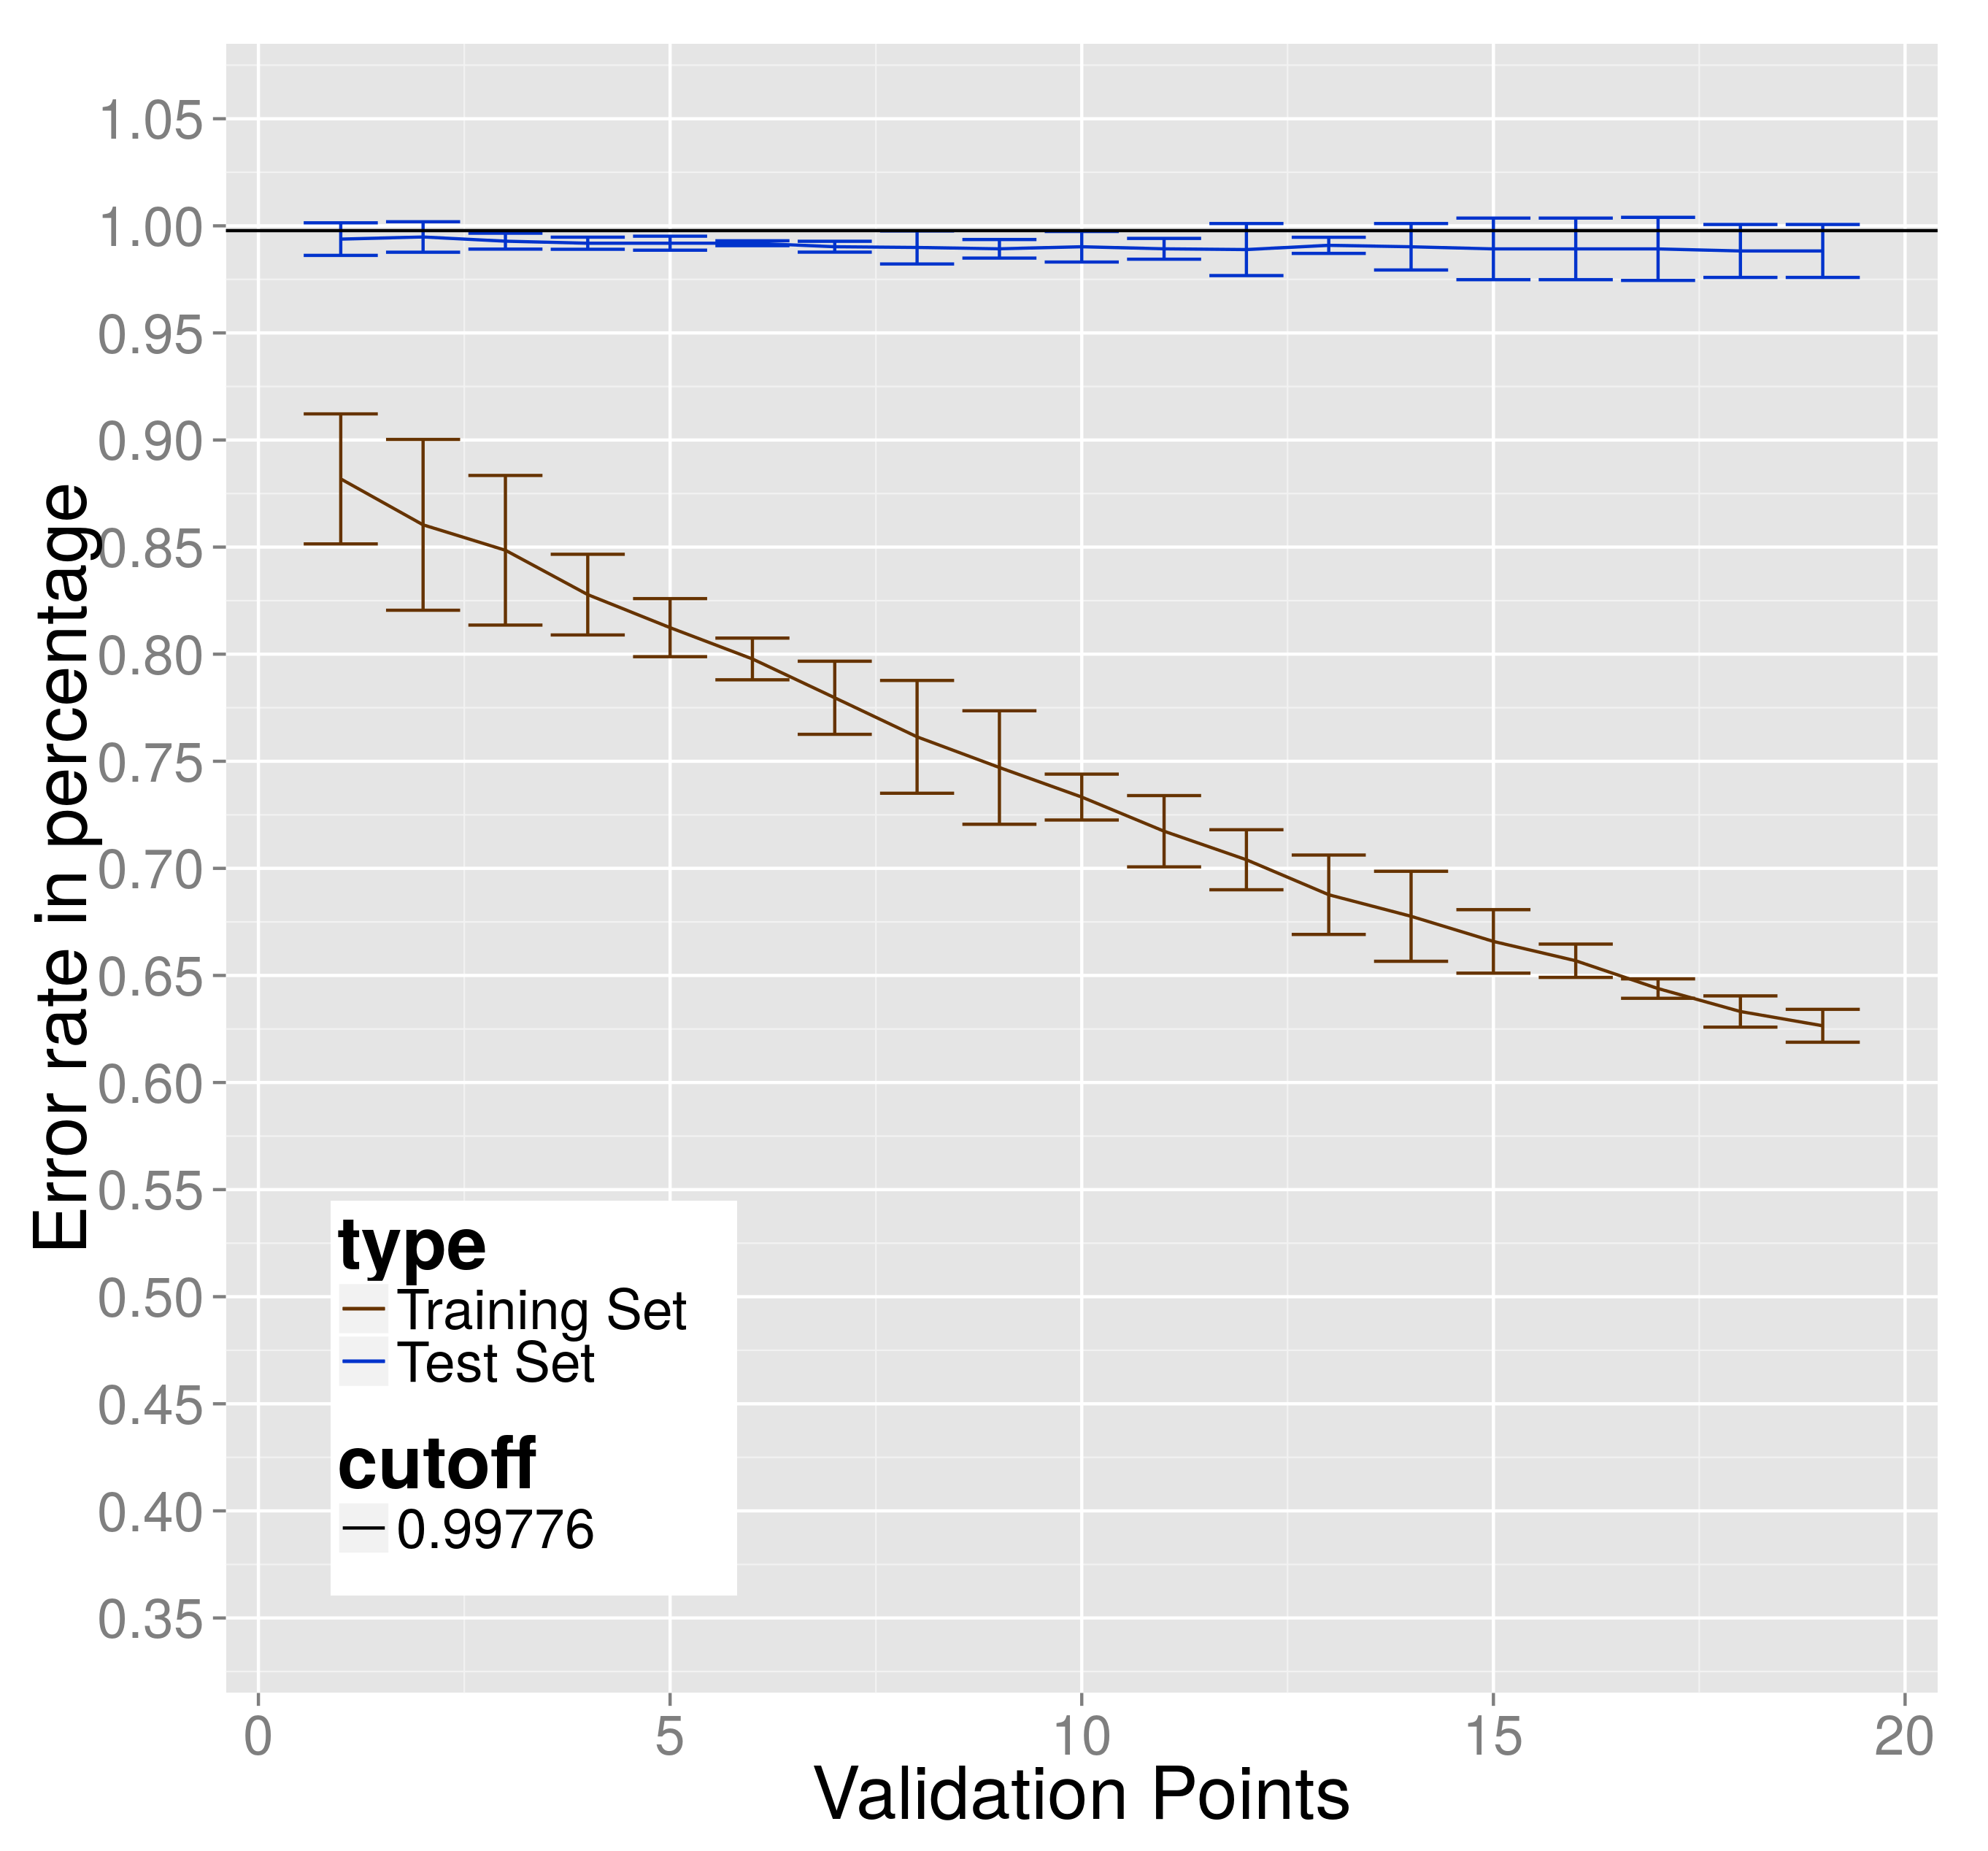
\includegraphics[width=0.9\linewidth]{Images/DRFpreprocessed}
  \caption{Random Forest - Preprocessed and Resized Images}
  \label{fig:rf-preprocessed}
\end{figure*}

\subsubsection{Neural Network}
\label{subsubsec:neuralnetwork}
This section contains the results from the neural network model using both the resized and the preprocessed and resized datasets.

\paragraph{The Resized Data}
in Figure \ref{fig:nn-resized} shows two non-static lines and a static cutoff line.
The static cutoff line represent random selection for a correct classification, where as the two other lines show the test and training sets performance against the model at given validation points. Additionally a one-tailed 95\% confident interval at 3 degrees of freedom is shown as the errorbar at each validation point for both lines.

The test set \emph{do not} have a significant better performance than random selection.

The training set do have a \emph{significant better performance} against the model compared to the test set, which shows overfitting also mentioned in \ref{par:rf-resized}

\begin{figure*}
  \centering
  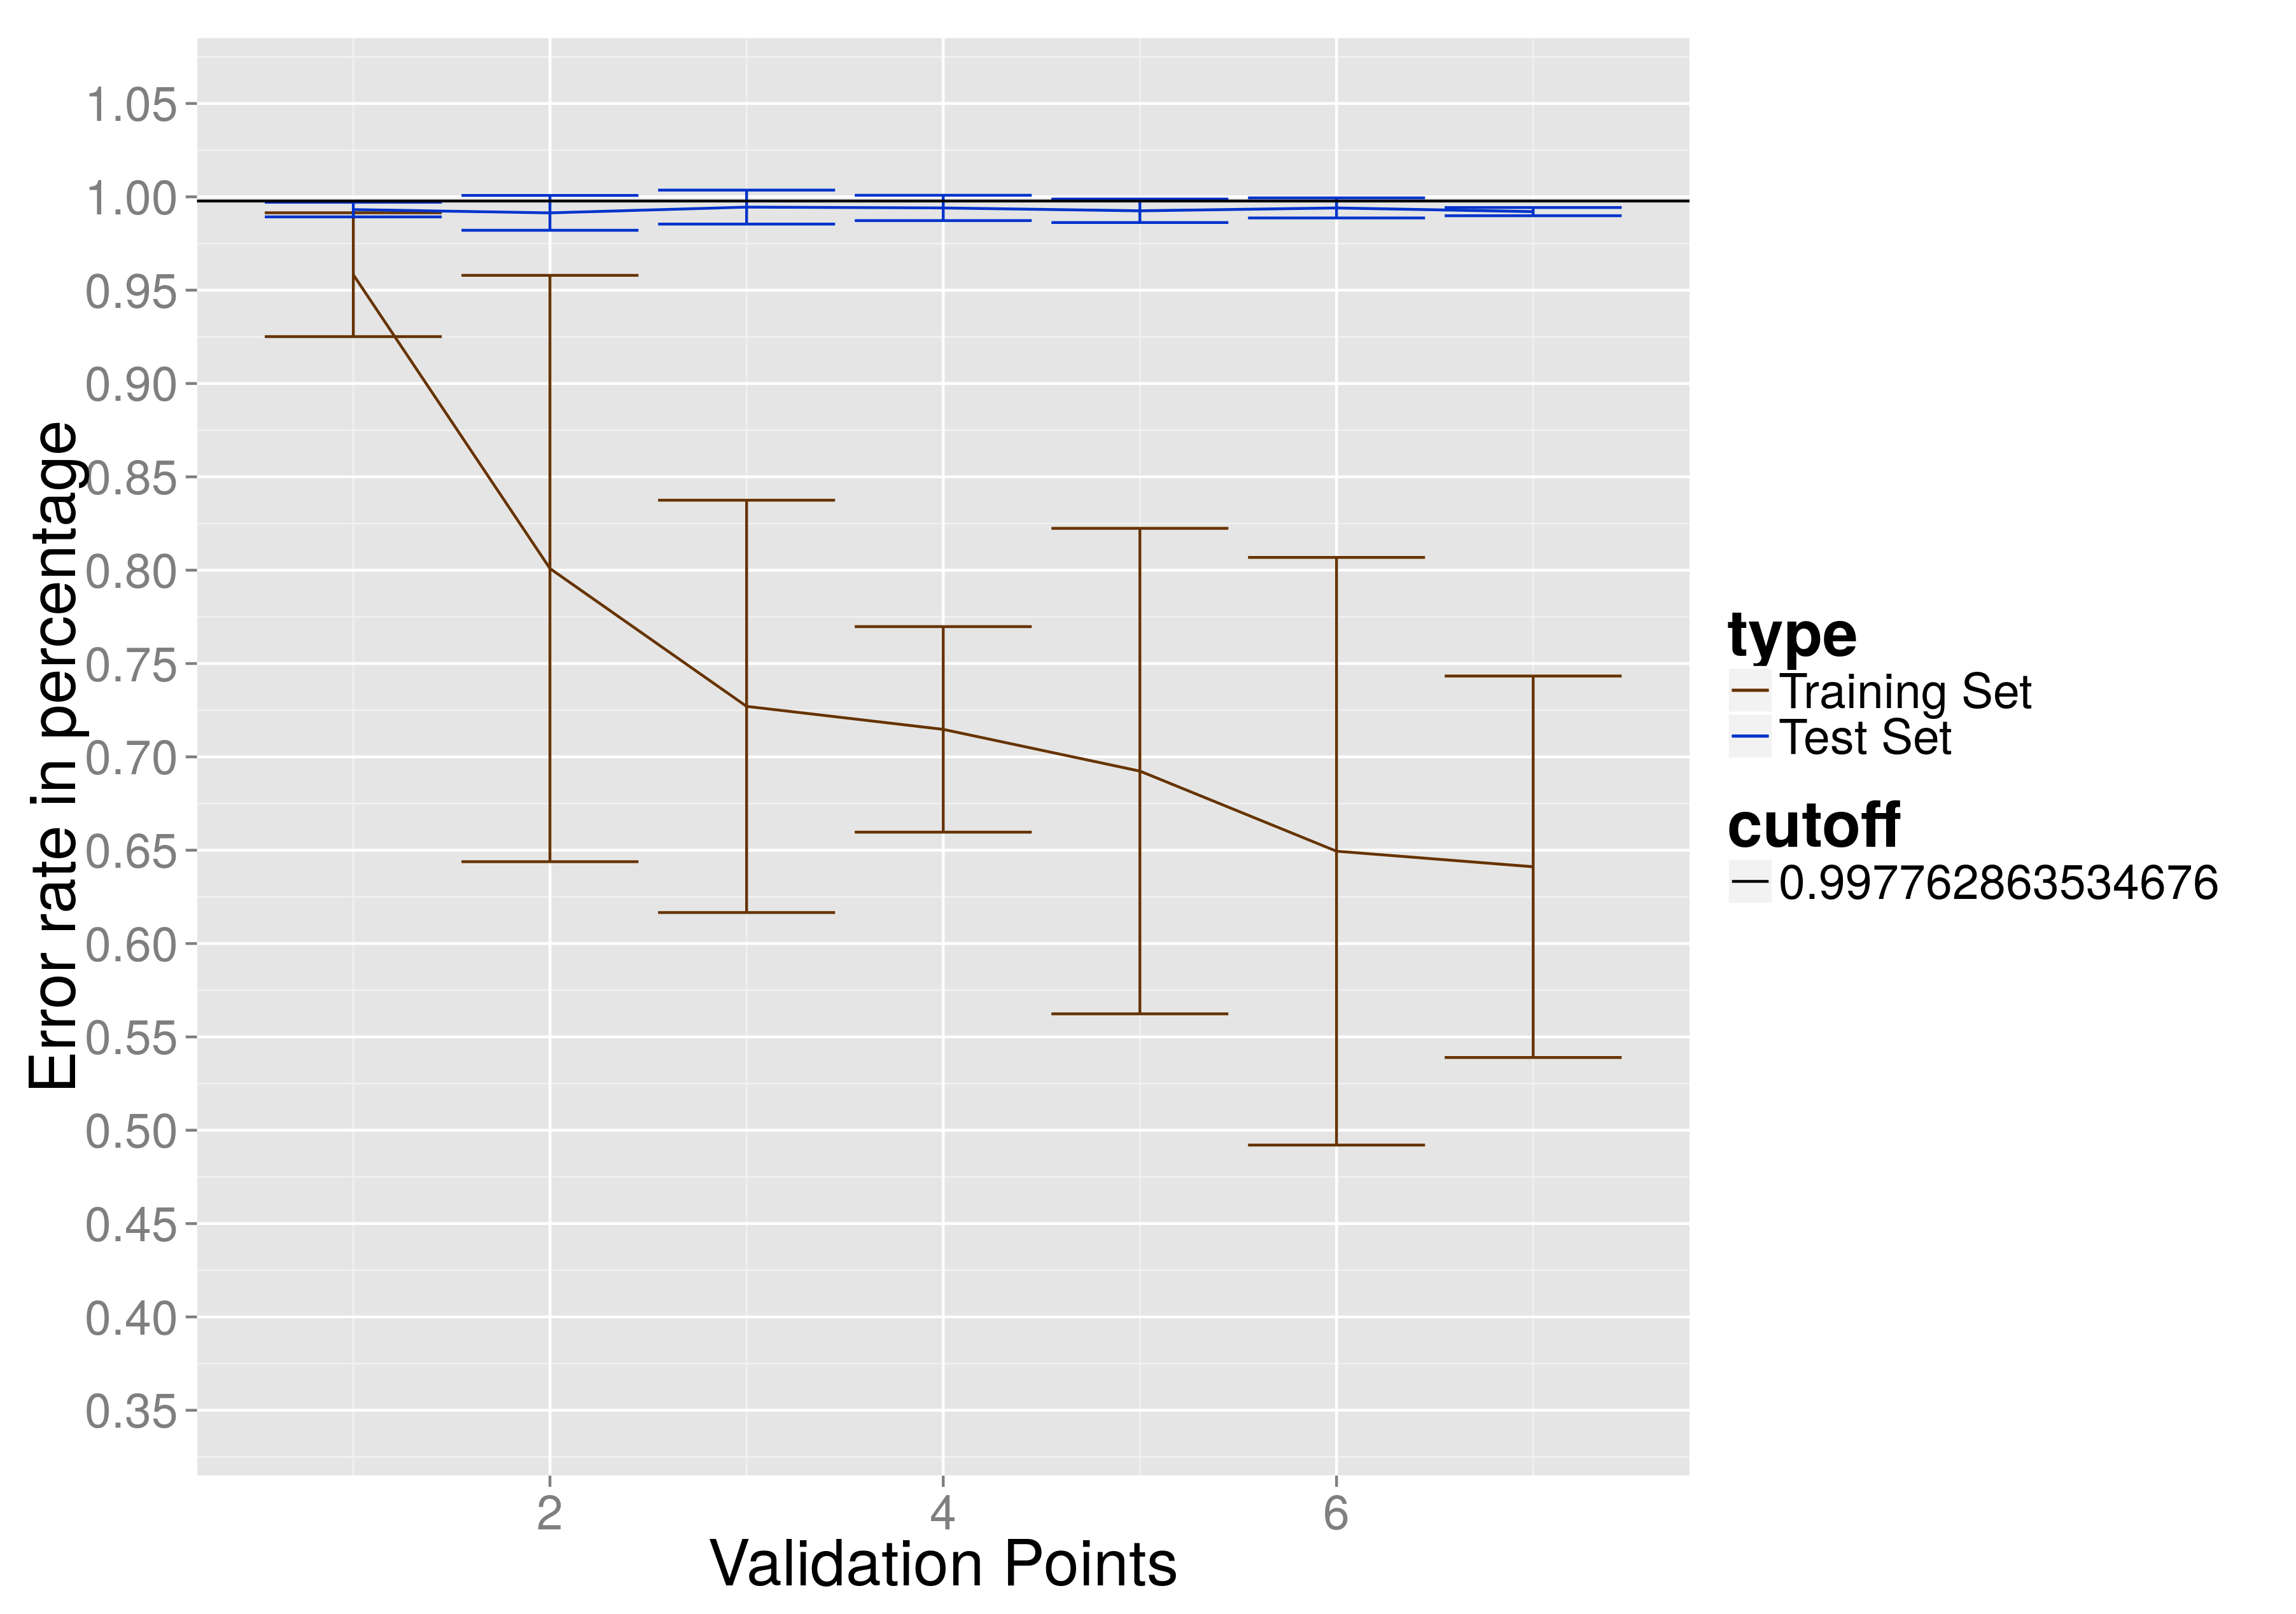
\includegraphics[width=0.9\linewidth]{Images/DNNraw}
  \caption{Neural Network - Resized Images}
  \label{fig:nn-resized}
\end{figure*}

\paragraph{The Preprocessed Data}
in Figure \ref{fig:nn-preprocssed} contains the same graph scheme as explained in previous paragraph in \ref{subsubsec:neuralnetwork}. 

The test set \emph{do not} have a significant better performance than random selection.

The training set do have a \emph{significant better performance} against the model compared to the test set.

\begin{figure*}
  \centering
  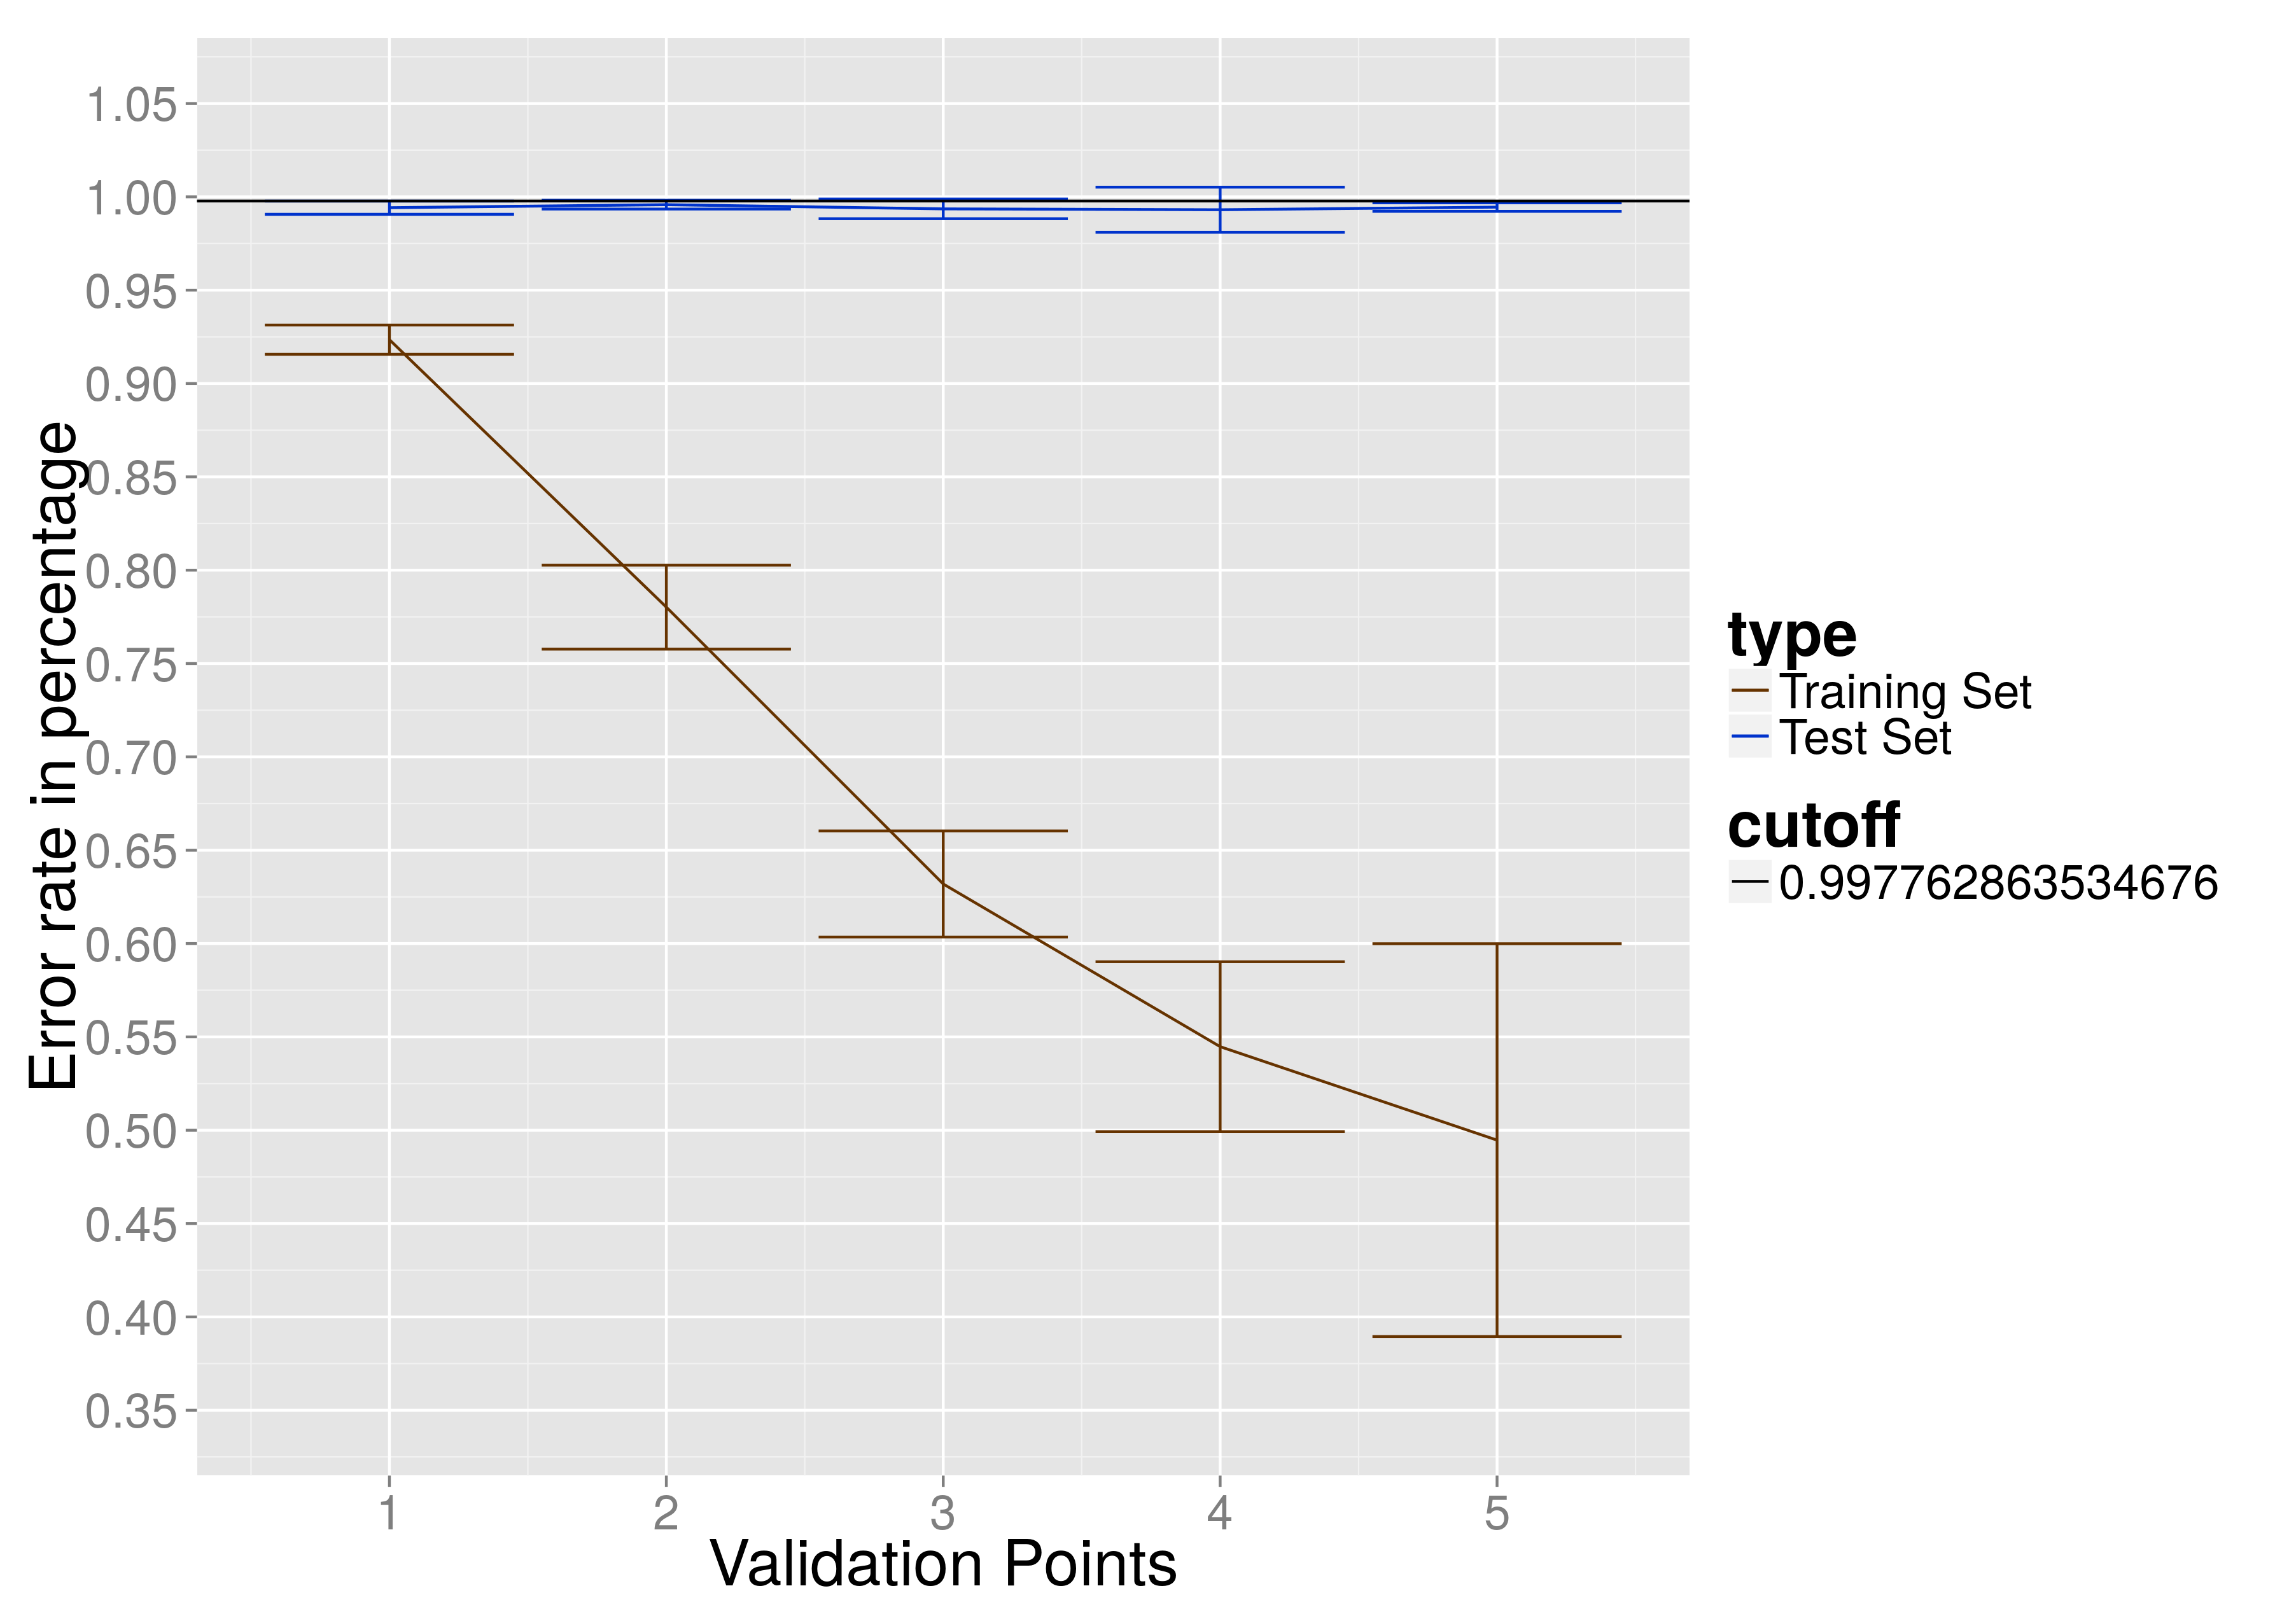
\includegraphics[width=0.9\linewidth]{Images/DNNpreprocessed}
  \caption{Neural Network - Preprocessed and Resized Images}
  \label{fig:nn-preprocessed}
\end{figure*}

\subsection{Evaluation}


\label{subsec:evaluation}